
\definecolor{c746c66}{RGB}{116,108,102}
\definecolor{cb3b3b3}{RGB}{179,179,179}
\definecolor{ccccccc}{RGB}{204,204,204}
\definecolor{c666666}{RGB}{102,102,102}
\definecolor{c999999}{RGB}{153,153,153}
\definecolor{c4d4d4d}{RGB}{77,77,77}
\definecolor{c7ed0e0}{RGB}{126,208,224}


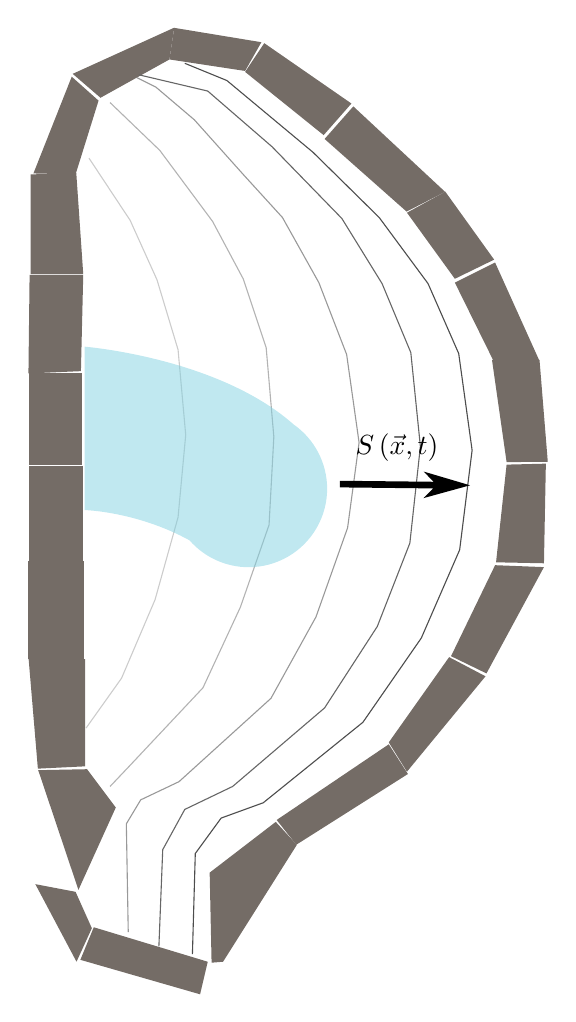
\begin{tikzpicture}[y=0.80pt, x=0.8pt,yscale=-1, inner sep=0pt, outer sep=0pt]
\begin{scope}[shift={(0,-579.86215)}]
  \path[fill=c746c66,line join=miter,line cap=butt,even odd rule,line
    width=1.327pt] (301.4139,795.2516) -- (294.8237,749.1138) --
    (316.2894,749.1138) -- (320.0172,795.0738) -- cycle;
  \path[fill=c746c66,line join=miter,line cap=butt,even odd rule,line
    width=1.327pt] (301.4139,796.3717) -- (319.1519,795.9390) --
    (318.2866,840.9330) -- (296.6549,840.5004) -- cycle;
  \path[fill=c746c66,line join=miter,line cap=butt,even odd rule,line
    width=1.327pt] (296.2223,841.7983) -- (276.3211,882.8986) --
    (292.3285,890.6860) -- (318.2866,842.6636) -- cycle;
  \path[fill=c746c66,line join=miter,line cap=butt,even odd rule,line
    width=1.327pt] (291.8959,891.9839) -- (275.4558,883.3312) --
    (248.1998,921.8357) -- (256.4081,935.0696) -- cycle;
  \path[fill=c746c66,line join=miter,line cap=butt,even odd rule,line
    width=1.327pt] (248.1998,922.7010) -- (197.5698,956.8791) --
    (206.4301,968.0623) -- (256.8525,936.1126) -- cycle;
  \path[fill=c746c66,line join=miter,line cap=butt,even odd rule,line
    width=1.327pt] (295.3570,749.2145) -- (316.1234,749.2145) --
    (296.2223,705.0858) -- (278.0516,714.1711) -- cycle;
  \path[fill=c746c66,line join=miter,line cap=butt,even odd rule,line
    width=1.327pt] (278.0516,712.4406) -- (256.4199,682.5888) --
    (273.7253,673.0709) -- (295.7896,703.7879) -- cycle;
  \path[fill=c746c66,line join=miter,line cap=butt,even odd rule,line
    width=1.327pt] (256.2421,682.0791) -- (219.2133,649.2759) --
    (232.1924,634.5664) -- (273.6482,673.1715) -- cycle;
  \path[fill=c746c66,line join=miter,line cap=butt,even odd rule,line
    width=1.327pt] (218.7807,647.5454) -- (231.3271,633.2685) --
    (191.9574,606.0125) -- (183.3047,618.9915) -- cycle;
  \path[fill=c746c66,line join=miter,line cap=butt,even odd rule,line
    width=1.327pt] (183.3047,618.5589) -- (149.1266,613.3673) --
    (151.2897,599.0904) -- (190.6595,605.5799) -- cycle;
  \path[fill=c746c66,line join=miter,line cap=butt,even odd rule,line
    width=1.327pt] (117.9769,630.6727) -- (105.4305,619.8568) --
    (151.3015,599.0133) -- (149.1265,613.3673) -- cycle;
  \path[fill=c746c66,line join=miter,line cap=butt,even odd rule,line
    width=1.327pt] (117.1116,631.9706) -- (104.9978,621.1547) --
    (87.6924,664.8508) -- (106.7284,665.2834) -- cycle;
  \path[fill=c746c66,line join=miter,line cap=butt,miter limit=4.00,line
    width=1.659pt] (107.0603,664.7619) -- (86.3945,665.2835) -- (86.3945,710.2774)
    -- (110.1895,710.2774) -- cycle;
  \path[fill=c746c66,line join=miter,line cap=butt,miter limit=4.00,line
    width=1.659pt] (110.1894,710.7100) -- (85.9619,710.7100) -- (85.4404,755.1943)
    -- (109.1464,754.1513) -- cycle;
  \path[fill=c746c66,line join=miter,line cap=butt,miter limit=4.00,line
    width=1.659pt] (109.7568,754.8388) -- (85.5293,754.8388) -- (85.5293,796.3717)
    -- (109.7568,796.3717) -- cycle;
  \path[fill=c746c66,line join=miter,line cap=butt,miter limit=4.00,line
    width=1.659pt] (110.1894,796.8043) -- (85.5293,796.8043) -- (85.5293,840.0677)
    -- (110.1894,840.0677) -- cycle;
  \path[fill=c746c66,line join=miter,line cap=butt,miter limit=4.00,line
    width=1.659pt] (110.6221,840.0677) -- (85.0967,840.0677) -- (85.0967,884.1965)
    -- (110.6221,884.1965) -- cycle;
  \path[fill=c746c66,line join=miter,line cap=butt,even odd rule,line
    width=1.327pt] (206.6669,968.1276) -- (173.3541,1020.9090) --
    (168.1625,1021.3416) -- (167.2972,980.6740) -- (197.1490,957.7443) -- cycle;
  \path[fill=c746c66,line join=miter,line cap=butt,even odd rule,line
    width=1.327pt] (166.4319,1020.9090) -- (114.9484,1005.3341) --
    (108.8915,1020.0437) -- (162.9708,1035.6185) -- cycle;
  \path[fill=c746c66,line join=miter,line cap=butt,even odd rule,line
    width=1.327pt] (114.0832,1005.7668) -- (106.7284,989.3267) --
    (88.5577,985.8656) -- (107.1610,1020.9090) -- cycle;
  \path[fill=c746c66,line join=miter,line cap=butt,even odd rule,line
    width=1.327pt] (108.0263,988.4614) -- (124.8990,951.2548) --
    (111.9200,933.9495) -- (89.8556,934.3821) -- cycle;
  \path[draw=cb3b3b3,line join=miter,line cap=butt,miter limit=4.00,even odd
    rule,line width=0.400pt] (122.3032,632.8358) -- (144.8002,654.4676) --
    (168.5951,686.4825) -- (182.4394,712.4406) -- (192.8226,743.5903) --
    (196.2837,783.8253) -- (194.1205,823.6276) -- (181.1415,860.8342) --
    (164.2688,897.1755) -- (130.5233,933.0842) -- (122.3032,941.7369);
  \path[draw=ccccccc,line join=miter,line cap=butt,miter limit=4.00,even odd
    rule,line width=0.400pt] (112.7853,657.9286) -- (131.3885,686.0499) --
    (143.5023,712.8732) -- (153.0203,744.4555) -- (156.4813,782.9600) --
    (153.0203,820.1666) -- (142.6370,857.3732) -- (127.4948,892.8492) --
    (111.4873,915.3462);
  \path[draw=c666666,line join=miter,line cap=butt,miter limit=4.00,even odd
    rule,line width=0.400pt] (135.2823,620.2894) -- (166.4319,627.6442) --
    (195.4184,652.7370) -- (227.0007,685.1846) -- (245.1714,714.6038) --
    (258.1504,745.7534) -- (262.4768,788.1516) -- (257.7178,831.8477) --
    (243.0082,869.4869) -- (219.2133,906.2609) -- (177.6804,941.7369) --
    (156.0487,952.1201) -- (146.0981,970.2907) -- (144.3676,1013.9868);
  \path[draw=c999999,line join=miter,line cap=butt,miter limit=4.00,even odd
    rule,line width=0.400pt] (130.5233,1007.4973) -- (129.6580,958.6096) --
    (136.1475,947.7937) -- (153.4529,939.5737) -- (194.9858,901.9345) --
    (215.3196,865.1606) -- (229.5965,824.9256) -- (234.7882,786.4211) --
    (229.1639,746.6187) -- (216.6175,714.1711) -- (200.1774,684.7520) --
    (182.4394,665.2834) -- (160.3750,640.6233) -- (143.0697,625.9137) --
    (134.4170,621.5873);
  \path[draw=c4d4d4d,line join=miter,line cap=butt,miter limit=4.00,even odd
    rule,line width=0.400pt] (159.5098,1017.4479) -- (160.8077,972.0213) --
    (172.4888,956.0138) -- (191.5247,949.0917) -- (236.5187,912.7504) --
    (262.9094,874.6785) -- (280.2148,834.8761) -- (285.8390,789.8822) --
    (279.7822,746.1861) -- (265.9379,714.6038) -- (243.8735,684.7520) --
    (214.0217,655.3329) -- (175.0846,622.8853) -- (156.0487,615.0978);
  \path[fill=c746c66,line join=miter,line cap=butt,miter limit=4.00,line
    width=1.659pt] (111.0547,884.1964) -- (85.5293,884.1964) -- (89.7015,933.6945)
    -- (111.0547,932.6515) -- cycle;
  \path[shift={(0,579.86215)},fill=c7ed0e0,line join=miter,line cap=butt,miter
    limit=4.00,fill opacity=0.490,line width=1.000pt] (110.8379,163.2363) --
    (110.8379,237.0332) .. controls (110.8379,237.0332) and (134.3853,237.6515) ..
    (158.1973,250.6914)arc(138.912:90.054:35.464)arc(90.002:0.001:35.464)arc(359.918:304.976:35.464)
    .. controls (171.1286,168.1394) and (110.8379,163.2363) .. (110.8379,163.2363)
    -- cycle;
  \path[color=black,fill=black,line join=miter,line cap=butt,miter limit=4.00,even
    odd rule,line width=2.400pt] (263.9523,799.5145) -- (284.8957,805.7098) --
    (263.8410,811.5125) -- (268.3175,807.1200) -- (226.0793,806.6610) --
    (226.1027,803.6610) -- (268.4757,804.1219) -- (263.9523,799.5145) -- cycle;
  \path[fill=black,line join=miter,line cap=butt,line width=0.800pt]
    (233.21275,794.72974) node[above right] (text4542)
    {$S\left(\vec{x},t\right)$};
\end{scope}

\end{tikzpicture}
